\documentclass[9pt,xcolor=dvipsnames]{beamer}
\usepackage[all]{xy}
\usepackage{animate}

\usepackage{amsmath}
\usepackage{amsfonts}
\usepackage{amsthm}

\newtheorem{proposition}{Proposition}
\newtheorem{remark}{Remark}
%\newtheorem{theorem}{Theorem}

% for figs from GeoGebra
\usepackage[utf8]{inputenc}
\usepackage{pgf,tikz}
\usetikzlibrary{arrows}
% end GeoGebra
\usepackage{listings}
\definecolor{codegreen}{rgb}{0,0.6,0}
\definecolor{codegray}{rgb}{0.5,0.5,0.5}
\definecolor{codepurple}{rgb}{0.58,0,0.82}
\definecolor{backcolour}{rgb}{0.95,0.95,0.92}
 
\lstdefinestyle{pystyle}{
    backgroundcolor=\color{backcolour},   
    commentstyle=\color{codegreen},
    keywordstyle=\color{magenta},
    numberstyle=\tiny\color{codegray},
    stringstyle=\color{codepurple},
    basicstyle=\footnotesize,
    breakatwhitespace=false,         
    breaklines=true,                 
    captionpos=b,                    
    keepspaces=true,                 
    numbers=left,                    
    numbersep=5pt,                  
    showspaces=false,                
    showstringspaces=false,
    showtabs=false,                  
    tabsize=2
}
\lstset{style=pystyle}

\usepackage{wrapfig}

%\usepackage[pdftex]{graphicx}
%\usepackage{epstopdf}
%\usepackage{graphicx}
\newtheorem{algorithm}[theorem]{Algorithm}
\newcommand{\Ropt}{\mathcal{R}}
\newcommand{\semfootnote}[1]{\let\thefootnote\relax\footnotetext{#1}}
%%%%%%%%%%%%%%%%%%%%%%%%%%%%%%%%%%%%%%%%%%%%%%%%%%%%%%%%%%
\definecolor{MyBlue}{rgb}{0.1,0.3,1} 
\definecolor{MyBlue2}{rgb}{0.1,0.3,0.6}
\definecolor{orange}{rgb}{0.5,0.5,0.}
\definecolor{darkblue}{rgb}{.1,.1,.1}
\definecolor{darkgreen}{rgb}{0.,.4,0.}

\mode<presentation>
{
\usetheme{Pittsburgh}
\usecolortheme{seahorse}
\setbeamertemplate{blocks}[rounded]
\setbeamercolor{title}{bg=MyBlue2,fg=white}
\setbeamercolor{frametitle}{bg=MyBlue2,fg=white}
%\setbeamercolor{section number projected}{bg=gray!50,fg=black}
\setbeamercolor{section in toc}{fg=black}
\setbeamercolor{block title}{fg=black,bg=darkgreen!70}
\setbeamercolor{block body}{fg=black,bg=darkgreen!10}
%\setbeamercolor{block title alerted}{fg=red,bg=darkgreen!40}
%\setbeamerfont{block title}{series=\bfseries, bg=Myblue}
\setbeamerfont{title}{size=\LARGE}
%
%\usefonttheme{serif}
}
%%%%%%%%%%%%%%%%%%%%%%%%%%%%%%%%%%%%%%%%%%%%%%%%%%%%%%%%%%
%\usepackage{remreset}
%\makeatletter
%\@removefromreset{subsection}{section}
%\makeatother
%\setcounter{subsection}{-1}
%%%%%%%%%%%%%%%%%%%%%%%%%%%%%%%%%%%%%%%%%%%%%%%%%%%%%%%%%%
%% extra definitions
%% September 2, 2013

% math definitions
\newcommand{\OM}{\Omega}
\newcommand{\RE}{\mathbb{R}}
\newcommand{\PO}{\mathbb{P}}
\newcommand{\NA}{\mathbb{N}}
\newcommand{\ra}{\mathfrak{r}}
\newcommand{\Dt}{\Delta t}
\newcommand{\Dx}{\Delta x}
\newcommand{\Dif}[2]{\frac{d {#1}}{d {#2}}}
\newcommand{\PDif}[2]{\frac{\partial {#1}}{\partial {#2}}}
%
\newcommand{\Lsp}{\textrm{L}}
\newcommand{\Hsp}{\textrm{H}}
\newcommand{\Tsp}{\textrm{T}}
%
\newcommand{\Uh}{\mathbf{u}_h}
\newcommand{\Uhbar}{\mathbf{\bar{u}}_h}
\newcommand{\Ufbar}{\mathbf{\bar{u}}_f}
\newcommand{\Ucbar}{\mathbf{\bar{u}}_c}
\newcommand{\Uf}{\mathbf{u}_f}
\newcommand{\Uc}{\mathbf{u}_c}
\newcommand{\Eh}{\mathbf{e}_h}
\newcommand{\Ef}{\mathbf{e}_f}
\newcommand{\Ec}{\mathbf{e}_c}
\newcommand{\DI}{\mathcal{D}}
\newcommand{\Arr}[2]{
	\left(
		\begin{array}{c}
		{#1} 
		%
		\\
		%
		{#2}
		\end{array}
	\right)
}
\newcommand{\Arrtri}[3]{
	\left(
		\begin{array}{c}
		{#1} 
		%
		\\
		%
		{#2}
		\\
		%
		{#3}		
		\end{array}
	\right)
}
\newcommand{\ARR}[4]{
	\left(
		\begin{array}{c}
		{#1} 
		%
		\\
		%
		{#2}
		\\
		{#3} 
		%
		\\
		%
		{#4}		
		\end{array}
	\right)
}
\newcommand{\MAT}[4]{
	\left[
		\begin{array}{c|c}
		{#1} 
		%
		&
		%
		{#2}
		\\ \hline
		{#3} 
		%
		&
		%
		{#4}		
		\end{array}
	\right]
}
\newcommand{\MATT}[4]{
	\left[
		\begin{array}{cc}
		{#1} 
		%
		&
		%
		{#2}
		\\
		{#3} 
		%
		&
		%
		{#4}		
		\end{array}
	\right]
}
\newcommand{\MATnine}[9]{
	\left[
		\begin{array}{ccc}
		{#1} & {#2} & {#3}
		\\
		{#4} & {#5} & {#6}
		%
		\\
		%
		{#7} & {#8} & {#9}		
		\end{array}
	\right]
}

\newcommand{\tA}{\tilde{A}}
\newcommand{\tB}{\tilde{B}}
\newcommand{\Ont}{\mathcal{O}}
\newcommand{\half}{\frac{1}{2}}

% Finite element, DG
%% jump - average operators
\newcommand{\average}[1]{\ensuremath{\lbrace\!\!\lbrace#1\rbrace\!\!\rbrace} } 
\newcommand{\jump}[1]{\ensuremath{[\![#1]\!]} }

\newcommand{\jumpF}[1]{\ensuremath{[\![\![#1]\!]\!]} }
\newcommand{\averageF}[1]{\ensuremath{\lbrace\!\lbrace\!\lbrace#1\rbrace\!\rbrace\!\rbrace} } 


\newcommand{\diff}{\varepsilon} %usata
%
\newcommand{\Th}{\mathcal{T}_h} %usata
\newcommand{\Thi}[1]{\mathcal{T}_{h,#1}} %usata
\newcommand{\Ti}[1]{\mathcal{T}_{#1}} %usata
%
\newcommand{\TAU}{{\boldsymbol \tau}}
\newcommand{\SIG}{{\boldsymbol \sigma} }
\newcommand{\BT}{{\boldsymbol \beta}}
\newcommand{\NOR}{{\boldsymbol n} }
\newcommand{\fB}{{\boldsymbol f} }
\newcommand{\vB}{{\boldsymbol v} }
\newcommand{\uB}{{\boldsymbol u} }
\newcommand{\wB}{{\boldsymbol w} }
\newcommand{\BO}[1]{{\boldsymbol #1} }
\newcommand{\lB}{{\boldsymbol \lambda} }
\newcommand{\phiB}{{\boldsymbol \varphi} }
\newcommand{\UDOF}{\underline{\boldsymbol u} }
\newcommand{\SDOF}{\underline{\boldsymbol \sigma} }
\newcommand{\Bopt}{\mathcal{B}}
\newcommand{\Hopt}{\mathcal{H}}
\newcommand{\Zopt}{{\boldsymbol \theta}}
%
\newcommand{\EPS}{ \mathcal{E} }
%
\newcommand{\GAMF}{ \Gamma^{ \mathtt{f} } }
\newcommand{\GAMI}{ \Gamma^{ 0 } }
\newcommand{\GAM}{ \Gamma }

%
\newcommand{\dotV}[2]{\left( {#1} , {#2} \right) }
\newcommand{\dotS}[2]{\left\langle #1 , #2 \right\rangle }

\newcommand{\Nel}{N_{\text{el} }}
\newcommand{\hmax}{h_{\text{max} }}
%\newcommand{\trin}[1]{{\left\vert\kern-0.25ex\left\vert\kern-0.25ex\left\vert #1 
%   \right\vert\kern-0.25ex\right\vert\kern-0.25ex\right\vert}}
\newcommand{\DGnorm}[2]{\Vert {#1} \Vert_{\textrm{\tt DG}{#2}} }
\newcommand{\Bnorm}[2]{\Vert {#1} \Vert_{{\tt HDG} #2} }
\newcommand{\Lnorm}[1]{{ \Vert #1 \Vert }}
\newcommand{\semin}[1]{\left| #1 \right|}

%\newcommand*{\defeq}{\mathrel{\vcenter{\baselineskip0.5ex \lineskiplimit0pt
%                                  \hbox{\scriptsize.}\hbox{\scriptsize.}}}=}
\newcommand{\norm}[1]{{ \Vert #1 \Vert }}


%
% Tikz configuration
\tikzset{
  every overlay node/.style={
    %draw=black,fill=white,rounded corners,
    anchor=north west, inner sep=0pt,
  },
}
% Usage:
% \tikzoverlay at (-1cm,-5cm) {content};
% or
% \tikzoverlay[text width=5cm] at (-1cm,-5cm) {content};
\def\tikzoverlay{%
   \tikz[remember picture, overlay]\node[every overlay node]
}%
%
\begin{document}
%
\date{Nov. 25, 2022}

\author[S. Hajian]{
	{Soheil Hajian}
	}
%
\institute[]
	{
	  %\inst{1}
	\vspace{1cm}
	{\normalsize\texttt{soheil.hajian@outlook.com}}
	}

\setbeamertemplate{navigation symbols}{} % get the rid of navigation symbols
\setbeamertemplate{footline}[frame number]
%
\title[]{Software testing: What, Why and How}

%
%\subtitle[]{Discontinuous Galerkin method}
%
%%%%%%%%%%%%%%%%%%%%%%%%%%%%%%%%%%%%%%%%%%%%%%%%%%%%%%%%%%
%
\begin{frame}[plain]
   %% \tikz [remember picture,overlay]
   %%  \node at
   %%      ([yshift=4.cm, xshift=-3cm]current page.south) 
   %%      %or: (current page.center)
   %%      {\includegraphics[]{figs/mesh/ddmesh5.jpg}};

\begin{titlepage}
\end{titlepage}
\vfill
\end{frame}

\begin{frame}{Outline}
    \tableofcontents
\end{frame}
%

\section{What is software testing, and why is it important?}
\begin{frame}
  \frametitle{What is software testing, and why is it important?}
  \begin{itemize}
  \item What is testing?
    \begin{itemize}
    \item \textbf{Software testing} is the process of verfiying that a
      software does what it is supposed to do.
    \item Verifiability implies some knowledge of \textbf{requirements} for that software
      or its components.
    \end{itemize}
    \pause 
  \item Why is testing important?
    \begin{itemize}
      \item A test is a certificate that the software (or a piece of
        it) behaves as expected.
      \item Ensures that future updates to the software do not break
        old behavior.
      \item Gives a sense of code reliability. 
    \end{itemize}
  \end{itemize}

\end{frame}

\section{Different levels of testing}
\begin{frame}
  \frametitle{Different levels of testing}
  It is common practice to split the testing into different
  levels. The most common splitting contains: \textbf{unit-}, \textbf{integration-}, and
  \textbf{system testing}.
  \vspace{1cm}
  \begin{center}
    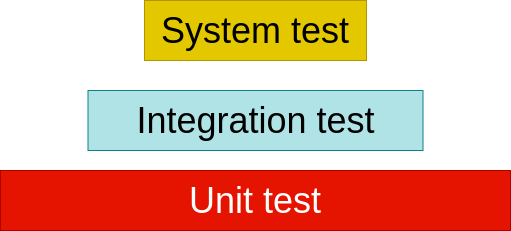
\includegraphics[scale=0.3]{figs/levels.png}
  \end{center}
\end{frame}

\begin{frame}
  \frametitle{Unit testing}
  \begin{itemize}
    \item \textbf{Unit testing} is usually referred to testing an
      \textbf{individual component} of the code, e.g., functions or methods of a class.
    \item \textbf{Example:} Write test for a function that takes a float as
      input and returns the score of the input.
      \pause
      \begin{itemize} 
      \item Code:
        \lstinputlisting[language=Python]{../testing_exercises/some_functions/square.py}
        \pause
      \item Test:
        \lstinputlisting[language=Python]{../tests/unit_tests/some_functions/test_square.py}
      \end{itemize}
  \end{itemize}
\end{frame}


\begin{frame}
  \frametitle{Integration testing}
  \begin{overlayarea}{\textwidth}{\textheight}
  \begin{itemize}
    \item \textbf{Integration testing} verifies if a group of
      smaller units within a software works as expected.
    \item \textbf{Example:} Write test for a function that takes
      credentials to connect to a database, runs a query and return the
      result as a dataframe.
      \begin{itemize}
      \item<only@1> Flowchart:
        \vspace{1cm}
        \begin{center}
          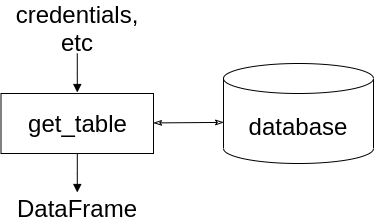
\includegraphics[scale=0.4]{figs/get_table.png}
        \end{center}
      \item<only@2> Code:
          \lstinputlisting[language=Python]{../testing_exercises/some_reader/read_db.py}
        \item<only@3> Test:
          \lstinputlisting[language=Python]{../tests/integration_tests/some_reader/test_reader_db.py}
      \end{itemize}
  \end{itemize}
  \end{overlayarea}
\end{frame}
\end{document}
%
